\documentclass[hidelinks]{article} % For LaTeX2e
\usepackage{iclr2016_conference,times}
\usepackage{hyperref}
\usepackage{url}
\usepackage{physics}
\usepackage{amsmath}
\usepackage{graphicx,import}
\usepackage[]{algorithm2e}

\title{The Incredible Shrinking Neural Network: Pruning to Operate in Constrained Memory Environments}

\author{Nikolas Wolfe, Aditya Sharma, Lukas Drude \& Bhiksha Raj \\
School of Computer Science\\
Carnegie Mellon University\\
Pittsburgh, PA 15213, USA \\
\texttt{\{nwolfe, adityasharma, bhiksha\}@cmu.edu}\\
\texttt{\{drude@nt.upb.de}\}
}

% The \author macro works with any number of authors. There are two commands
% used to separate the names and addresses of multiple authors: \And and \AND.
%
% Using \And between authors leaves it to \LaTeX{} to determine where to break
% the lines. Using \AND forces a linebreak at that point. So, if \LaTeX{}
% puts 3 of 4 authors names on the first line, and the last on the second
% line, try using \AND instead of \And before the third author name.

\newcommand{\fix}{\marginpar{FIX}}
\newcommand{\new}{\marginpar{NEW}}
\newcommand{\Out}[2]{o_{#1}^{(#2)}}
\newcommand{\Target}[1]{t_{#1}}
\newcommand{\Input}[2]{x_{#1}^{(#2)}}
\newcommand{\Weight}[3]{w_{#1#2}^{(#3)}}
\newcommand{\Con}[3]{c_{#1#2}^{(#3)}}
\newcommand{\Etotal}{E_{\mathrm{total}}}

\setlength{\parindent}{0pt}

%\iclrfinalcopy % Uncomment for camera-ready version

\begin{document}


\maketitle

\begin{abstract}
We propose and evaluate a method for pruning neural networks to operate in constrained memory environments such as mobile or embedded devices. We evaluate a simple pruning technique using first-order derivative approximations of the gradient of each neuron in an optimally trained network, and turning off those neurons which contribute least to the output of the network. We then show the limitations of this type of approximation by comparing against the ground truth value for the change in error resulting from the removal of a given neuron. We attempt to improve on this using a second-order derivative approximation. We also explore the correlation between neurons in a trained network and attempt to improve our choice of candidate neurons for removal to account for faults that can occur from the removal of a single neuron at a time. We argue that this method of pruning allows for the optimal tradeoff in network size versus accuracy in order to operate within the memory constraints of a particular device or application environment. 
\end{abstract}
\section{Introduction}
Neural network pruning algorithms were first popularized by \cite{sietsma1988neural} as a mechanism to determine the size of network required to solve a particular problem. To this day, network design and optimal pruning remain inherently difficult tasks. For problems which cannot be solved using linear threshold units alone, \cite{baum1989size} demonstrate there is no way to precisely determine the appropriate size of a neural network a priori given any random set of training instances. Using too few neurons inhibits learning, and so in practice it is common to attempt to over-parameterize networks initially using a large number of hidden units and weights. However, as \cite{chauvin1990generalization} writes, this approach can lead to overfitting as the network starts to latch on to idiosyncrasies in the training data. 


Pruning algorithms, as comprehensively surveyed by \cite{reed1993pruning}, are a useful set of heruristics designed to identify and remove network parameters which do not contribute significantly to the output of the network and potentially inhibit generalization performance. At the time of Reed's writing, reducing network size was also a practical concern, as smaller networks are preferable in situations where computational resources are scarce. In this paper we are particularly concerned with application domains in which space is limited and network size constraints must be imposed with minimal impact on performance.


The generalization performance of neural networks has been well studied, and apart from pruning algorithms many heuristics have been used to avoid overfitting, such as dropout (\cite{srivastava2014dropout}), maxout (\cite{goodfellow2013maxout}), and cascade correlation (\cite{fahlman1989cascade}), among others. However, these algorithms do not prioritize the reduction of network memory footprint as an explicit part of their optimization criteria per se, (although cascade correlation holds promise in this regard.) Computer memory size and processing capabilities have improved so much since the introduction of pruning algorithms that space complexity has become an almost negligible concern. The proliferation of Cloud-based computing services has furthermore enabled mobile and embedded devices to leverage the power of massive data and computing centers remotely. It is of course conceivable, however, that performance-critical applications running on low-resource devices could benefit immensely from the ability to use powerful neural networks locally. 


Unfortunately, at present there are few if any mechanisms to shrink neural networks down in order to meet an externally imposed constraint on byte-size in memory. Arguably one could accomplish this using any number of off-the-shelf pruning algorithms, such as Skeletonization (\cite{mozer1989skeletonization}), Optimal Brain Damage (\cite{lecun1989optimal}), or later variants such as Optimal Brain Surgeon (\cite{hassibi1993second}). In fact, we borrow much of our inspiration from these antecedent algorithms, with one major variation. 


The aforementioned strategies all focus on the targeting and removal of \textit{weight} parameters. Scoring and ranking individual weight parameters is computationally expensive, and generally speaking the removal of a single weight from a large network is a drop in the bucket in terms of reducing a network's core memory footprint. We therefore train our sights on the ranking and removal of entire neurons along with their associated weight parameters. We argue that this is more efficient computationally as well as practically in terms of quickly reaching a target reduction in memory size. Our approach also attacks the angle of giving downstream applications a realistic expectation of the minimal increase in error resulting from the removal of a specified percentage of neurons from a trained network. Such trade-offs are unavoidable, but performance impacts can be limited if a principled approach is used to find candidate neurons for removal. 



\section{Methodology}
The general approach taken to prune an optimally trained neural network in the present work is to create a ranked list of all the neurons in the network based off of one of the 3 ranking criteria: Brute Force approximation (which we use as our ground truth), linear approximation and quadratic approximation. We then test the effects of removing neurons sequentially on the accuracy of the network. These tests can be found in the Experiments section. Next, we propose our algorithm: The Gain-Switch and compare its performance to the first method.

\subsection{Brute Force Removal Approach}
This is perhaps the most naive yet the most accurate method for pruning the network. It is also the slowest and hence unusable on large-scale neural networks with thousands of neurons. The idea is to manually check the effect of every single neuron on the output. This is done by running a forward propagation on the validation set $K$ times (where $K$ is the total number of neurons in the network), turning off exactly one neuron each time (keeping all other neurons active) and noting down the change in error. Turning a neuron off can be achieved by simply setting its output to 0. This results in all the outgoing weights from that neuron being turned off. This change in error is then used to generate the ranked list. 

\subsubsection{Taylor Series Representation of Error}
Let us denote the total error from the optimally trained neural network for any given validation dataset with $N$ instances as $\Etotal$. Then,
\begin{align}
\Etotal = \sum _n E_n,
\end{align}
where $E_n$ is the error from the network over one validation instance. $E_n$ can be seen as a function $O$, where $O$ is the output of any general neuron in the network (In reality this error depends on each neuron's output, but for the sake of simplicity we use $O$ to represent that). This error can be approximated at a particular neuron's output (say $O_k$) by using the 2nd order Taylor Series as,

\begin{align}
\hat E_n(O) \approx E_n(O_k) + (O-O_k)\cdot E_n(O_k) + \left.\pdv{E_n}{O}\right|_{O_k} +  0.5\cdot (O-O_k)^2\cdot \left.\pdv[2]{E_n}{O}\right|_{O_k}\label{eq:ts1},
\end{align}

where $\hat E_n(O_k)$ represents the contribution of a neuron $k$ to the total error $E_n$ of the network for any given validation instance $n$. When this neuron is pruned, its output $O_k$ becomes 0. From equation \ref{eq:ts1}, the contribution $E_n(0)$ of this neuron, then becomes:

\begin{align}
\hat E_n(0) \approx E_n(O_k) - O_k\cdot \left.\pdv{E_n}{O}\right|_{O_k} +  0.5\cdot O_k^2\cdot \left.\pdv[2]{E_n}{O}\right|_{O_k}\label{eq:ts2}
\end{align}

Replacing $O$ by $O_k$ in equation \ref{eq:ts1} shows us that the error is approximated perfectly by equation \ref{eq:ts1} at $O_k$. Using this and equation \ref{eq:ts2} we get:

\begin{align}
\Delta E_{n,k} = \hat E_n(0) - \hat E_n(O_k)= - O_k\cdot \left.\pdv{E_n}{O}\right|_{O_k} + 0.5\cdot O_k^2\cdot \left.\pdv[2]{E_n}{O}\right|_{O_k}\label{eq:ts3},
\end{align}

where $\Delta E_{n,k}$ is the change in the total error of the network given a validation instance $n$, when exactly one neuron ($k$) is turned off.


\subsection{Linear Approximation Approach}
\begin{figure}[bh!]
\centering
\newcommand{\repSigmoid}{$\sigma(\cdot)$}
\newcommand{\repLinear}{$\sum$}
\newcommand{\repMse}{MSE}
\newcommand{\repFirstSum}{$\Input j 1$}
\newcommand{\repLastSum}{$\Input i 0$}
\newcommand{\repFirstOutput}{\hspace{1.5cm}$\Con j i 0 \!=\! \Weight j i 0 \Out j 1$}
\newcommand{\repLastOutput}{$\Out i 0$}
\newcommand{\repLoss}{$E$}
\def\svgwidth{0.9\textwidth}
\hspace{-2cm}
\import{}{drawing.pdf_tex}
\hspace{-2cm}
\caption{Simple feed-forward network illustrating the naming of different variables, where $\sigma(\cdot)$ is the nonlinearity, MSE is the mean-squared error cost function and $E$ is the overall loss.}
\end{figure}
We define the following network terminology here which will be used in this section and all subsequent sections  unless stated otherwise. Figure \ref{fig:comp_graph} can be used as a reference to the terminology defined here:

\begin{align}
E &= \frac{1}{2}\sum\limits_i (\Out i 0 - \Target i)^2 &
\Out i m &= \sigma(\Input i m) &
\Input i m &= \sum\limits_j {\Weight j i m}{ \Out j {m + 1}} &
\Con j i m = \Weight j i m \Out j {m+1}\label{eq:term}
\end{align}
Superscripts represent the index of the layer of the network in question, with 0 representing the output layer. $E$ is the squared-error network cost function. Note that we are dropping the $E_n$ notation used previously as the subsequent discussion is insusceptible to the data instances. $\Out i m$ is the $i$th output in layer $m$ generated by the activation function $\sigma$, which in this paper is is the standard logistic sigmoid. $\Input i m$ is the weighted sum of inputs to the $i$th neuron in the $m$th layer, and $\Con j i m$ is the contribution of the $j$th neuron in the $(m+1)$th layer to the input of the $i$th neuron in the $m$th layer. $\Weight j i m$ is the weight between the $j$th neuron in the $(m+1)$th layer and the $i$th neuron in the $m$th layer.

We can use equation \ref{eq:ts3} to get the linear error approximation of the change in error due to the $k$th neuron being turned off and represent it as $\Delta E_{k}^1$ as follows:

\begin{align}
\Delta E_{k}^1 = - o_k\cdot \left.\pdv{E}{{\Out j {m+1}}}\right|_{o_k}
\end{align}

The derivative term above is the first-order gradient which represents the change in error with respect to the output of a given neuron $o_j$ in the $(m+1)$th layer. This term can be collected during back-propagation. The derivative term above can be calculated as follows:

\begin{align}
\pdv{E}{{\Out j {m+1}}} = \sum\limits_i \pdv{E}{\Input i m}\cdot \Weight j i m
\end{align}

The full step-by-step mathematical derivation of the above equation can be found in the appendix.
\subsection{Quadratic Approximation Approach}

As seen in equation \ref{eq:ts3}, $\Delta E_{n,k}$ which can now be represented as $\Delta E_{k}^2$ is the quadratic approximation of the change in error due to the $k$th neuron being turned off. The quadratic term in equation \ref{eq:ts3} requires some discussion which we provide here. A more detailed and step-by-step mathematical derivation can be found in the appendix.

Let us reproduce equation \ref{eq:ts3} in our new terminology here: 
\begin{align}
\Delta E_{k}^2 = - o_k\cdot \left.\pdv{E}{{\Out j {m+1}}}\right|_{o_k} + 0.5\cdot o_k^2\cdot \left.\pdv[2]{E}{{\Out j {m+1}}}\right|_{o_k}\
\end{align}

The second term here involves the second-order gradient which represents the second-order change in error with respect to the output of a given neuron $o_j$ in the $(m+1)$th layer. This term can be generated by performing back-propagation using second derivatives. A full derivation of the second derivative back-propagation can be found in the appendix. We will quote some results from the derivation here. The second-order derivative term can be represented as:

\begin{align}
\pdv[2]{E}{{\Out j {m+1}}} &= \sum_i
\pdv[2]{E}{{\Con j i m}} \left({\Weight j i m}\right)^2
\end{align} 

Here,$\Con j i m$ is one of the component terms of $\Input i m$, as follows from the equations in \ref{eq:term}. Hence, it can be easily proved that (full proof in appendix):
\begin{align}
\pdv[2]{E}{{\Con j i m}} = \pdv[2]{E}{{\Input i m}}
\end{align}

Now, the value of $\Input i m$ can be easily calculated through the steps of the second-order back-propagation using Chain Rule. The full derivation can again, be found in the appendix.
\begin{align}
\pdv[2]{E}{{\Input i m}}=\pdv[2]{E}{{\Out i m}} \left(\sigma^{\prime}\left({\Input i m}\right)\right)^2
+
\pdv{E}{{\Out i m}}\sigma^{\prime\prime}\left(\Input i m\right)
\end{align}

\subsection{Pruning Algorithm: The Gain-switch}
We propose the Gain-switch algorithm for pruning an optimally trained neural network here. We define gain as the quadratic error approximation $\Delta E_{k}^2$ we got from the Taylor Series.

The first step is to  decide a stopping criterion. This can vary depending on the application but some intuitive stopping criteria can be the maximum number of neurons to remove, percentage scaling needed, maximum allowable accuracy drop etc. The Gain-switch algorithm performs the pruning in a greedy manner. It performs a forward propagation followed by a second-order back-propagation and collects the linear and quadratic gradients. It is to be noted that there is no weight update taking place during the back-propagation step as the network is already trained.This step is only used to collect the gradients. The algorithm then ranks all the neurons in the network based on their respective gain values and removes the neuron with the least value of the gain. 

\begin{algorithm}[H]
 \KwData{optimally trained network, training set}
 \KwResult{A pruned network after applying the Gain-switch algorithm}
 initialize and define stopping criterion \;
 \While{stopping criterion is not met}{
 $gain$ = $\Delta E_{k}^2$ \;
  perform forward propagation over the training set \;
  perform second-order back-propagation without updating weights and collect linear and quadratic gradients \;
  rank the remaining neurons based on $gain$ \;
  remove the neuron with the least value of $gain$ \;
 }
 \caption{The proposed Gain-switch pruning algorithm}
\end{algorithm}

The advantage of taking a greedy approach is that while removing the neurons, we are take into account the dependencies the neurons might have with one another. 

\section{Experiments}
\section{Experimental Results}

\begin{figure}
\centering
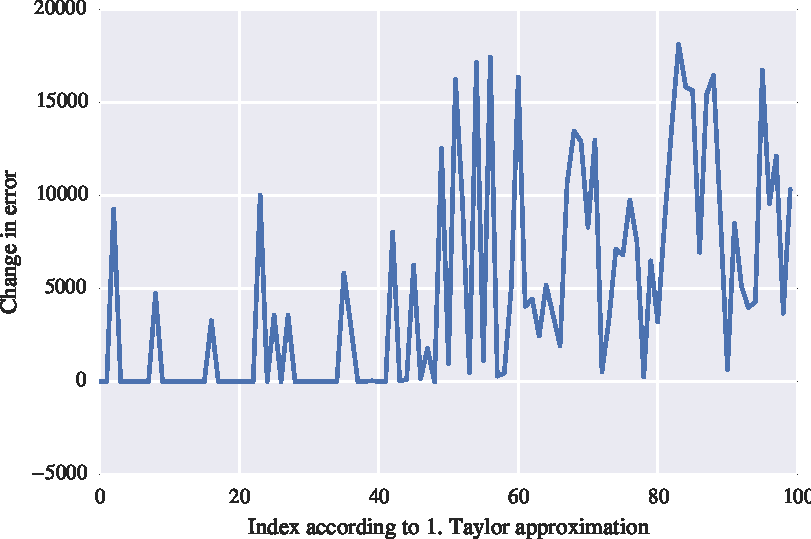
\includegraphics[width=0.6\linewidth]{error1.pdf}
\caption{Error when using first order Taylor Series approximation.}
\label{fig:error1}
\end{figure}

\begin{figure}
\centering
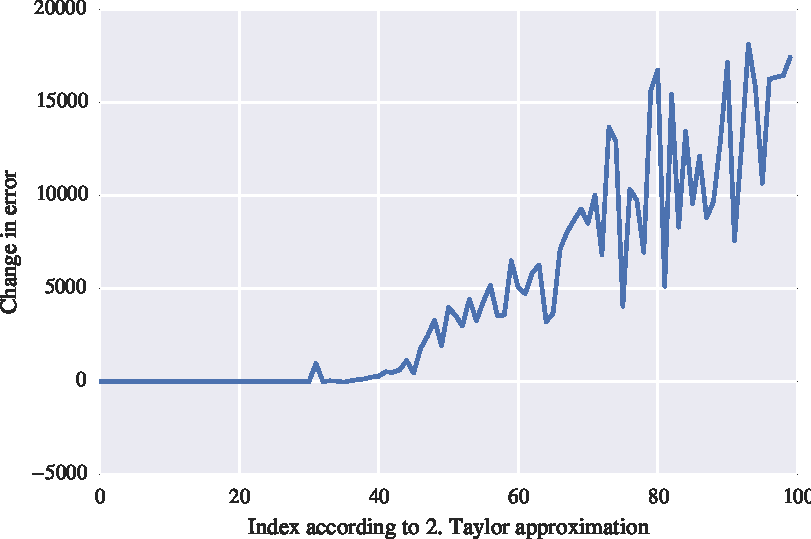
\includegraphics[width=0.6\linewidth]{error2.pdf}
\caption{Error when using second order Taylor Series approximation.}
\label{fig:error2}
\end{figure}

\begin{figure}
\centering
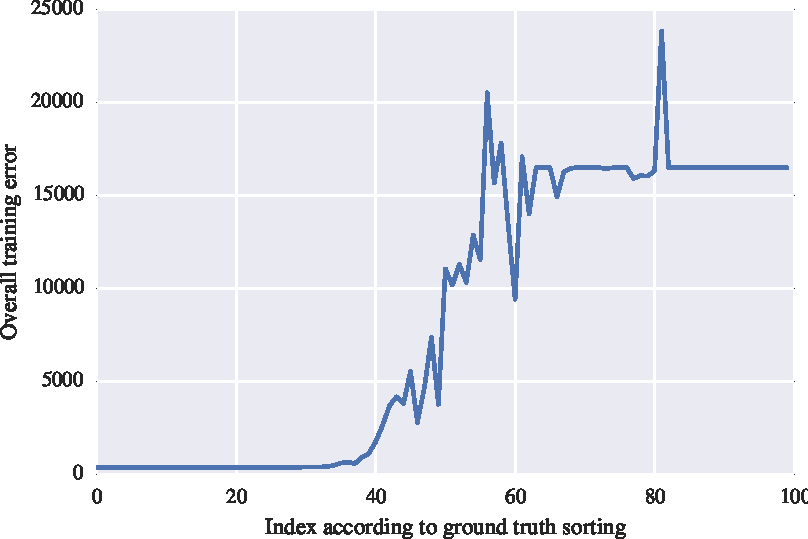
\includegraphics[width=0.6\linewidth]{improvement1.pdf}
\caption{Improvement of the training error when using the brute force ordering.}
\label{fig:improvement1}
\end{figure}

\begin{figure}
\centering
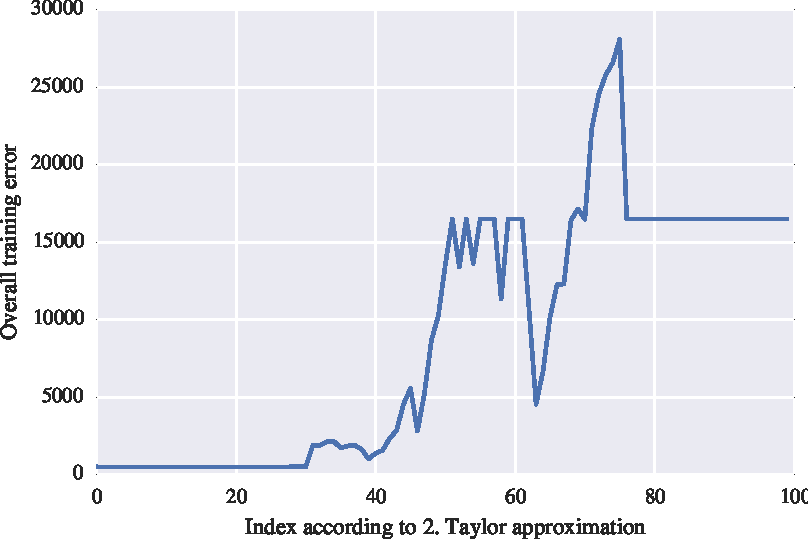
\includegraphics[width=0.6\linewidth]{improvement3.pdf}
\caption{Improvement of the training error when using the second order Taylor approximation.}
\label{fig:improvement3}
\end{figure}

\section{Conclusions}
\pagebreak
\section{Second Derivative Back-Propagation}
Name and network definitions:\\[5pt]
\begin{align}
E &= \frac{1}{2}\sum\limits_i (\Out i 0 - \Target i)^2 &
\Out i m &= \sigma(\Input i m) &
\Input i m &= \sum\limits_j {\Weight j i m}{ \Out j {m + 1}} &
\Con j i m = \Weight j i m \Out j {m+1}
\end{align}
Superscripts represent the index of the layer of the network in question, with 0 representing the output layer. $E$ is the squared-error network cost function. $\Out i m$ is the $i$th output in layer $m$ generated by the activation function $\sigma$, which in this paper is is the standard logistic sigmoid. $\Input i m$ is the weighted sum of inputs to the $i$th neuron in the $m$th layer, and $\Con j i m$ is the contribution of the $j$th neuron in the $m+1$ layer to the input of the $i$th neuron in the $m$th layer. 
\subsection{First and Second Derivatives} 
The first and second derivatives of the cost function with respect to the outputs:
\begin{align}
\pdv{E}{\Out i 0} &= \Out i 0 - \Target i \label{cost_func_derivative}
\end{align}
\begin{align}
\pdv[2]{E}{{\Out i 0}} &= 1\label{cost_func_2nd_derivative}
\end{align}
\\[5pt]
The first and second derivatives of the sigmoid function in forms depending only on the output:
\begin{align}
\sigma\prime(x) &= \sigma(x)\left(1 - \sigma(x)\right)\label{sigmoid_derivative} 
\\
\sigma\prime\prime(x) &= \sigma\prime(x)\left(1 - 2\sigma(x)\right) \label{sigmoid_2nd_derivative}
\end{align}
The second derivative of the sigmoid is easily derived from the first derivative:
\begin{align}
\sigma\prime(x) &= \sigma(x)\left(1 - \sigma(x)\right)
\\
\sigma\prime\prime(x) &= \dv{}{x}
\underbrace{\sigma(x)}_{f(x)}
\underbrace{\left(1 - \sigma(x)\right)}_{g(x)}
\\
\sigma\prime\prime(x) &= f\prime(x)g(x) + f(x)g\prime(x)
\\
\sigma\prime\prime(x) &= \sigma\prime(x)(1-\sigma(x)) - \sigma(x)\sigma\prime(x)
\\
\sigma\prime\prime(x) &= \sigma\prime(x) - 2\sigma(x)\sigma\prime(x)
\\
\sigma\prime\prime(x) &= \sigma\prime(x)(1 - 2\sigma(x))
\end{align}
And for future convenience: 
\begin{align}
\dv{\Out i m}{\Input i m} &= 
\dv{}{\Input i m}\left({\Out i m} = \sigma(\Input i m)\right) 
\\
&= \left(\Out i m\right)\left(1 - \Out i m\right)
\\
&= \sigma\prime\left(\Input i m\right)
\\
\dv[2]{{\Out i m}}{{\Input i m}} &=
\dv{}{{\Input i m}}\left(\dv{\Out i m}{\Input i m} = \left(\Out i m\right)\left(1 - \Out i m\right)\right)
\\
&= \left(\Out i m\left(1 - \Out i m\right)\right)\left(1 - 2\Out i m\right)
\\
&= \sigma\prime\prime\left(\Input i m\right)
\end{align}
\\[5pt]Derivative of the error with respect to the $i$th neuron's input $\Input i 0$ in the output layer:
\begin{align}
\pdv{E}{\Input i 0} &= \pdv{E}{\Out i 0} \pdv{\Out i 0}{\Input i 0} 
\\
&= \underbrace{\left(\Out i 0 - \Target i\right)}_{\text{from} \ (\ref{cost_func_derivative})} \underbrace{\sigma\left(\Input i 0\right)\left(1 - \sigma\left(\Input i 0\right)\right)}
_{\text{from} \ (\ref{sigmoid_derivative})}
\\
&= \left(\Out i 0 - \Target i\right)\left(\Out i 0 \left(1 - \Out i 0\right)\right)
\\
&= \left(\Out i 0 - \Target i\right)\sigma\prime\left(\Input i 0\right)\label{dedx}
\end{align}
\\[5pt]Second derivative of the error with respect to the $i$th neuron's input $\Input i 0$ in the output layer:
\begin{align}
\pdv[2]{E}{{\Input i 0}} &= \pdv{}{\Input i 0}
\left(\pdv{E}{\Out i 0}\pdv{\Out i 0}{\Input i 0}\right) 
\\
&= \pdv{{^2}E}{{\Input i 0}{\Out i 0}}\pdv{\Out i 0}{\Input i 0} + \pdv{E}{\Out i 0}\pdv[2]{\Out i 0}{{\Input i 0}}
\\
&= \pdv{{^2}E}{{\Input i 0}{\Out i 0}}\underbrace{\left(\Out i 0 \left(1 - \Out i 0\right)\right)}_{{\text{from} \ (\ref{sigmoid_derivative})}} + \underbrace{\left(\Out i 0 - \Target i\right)}_{\text{from} \ (\ref{cost_func_derivative})}\underbrace{\left(\Out i 0 \left(1 - \Out i 0\right)\right)\left(1 - 2\Out i 0\right) }_{\text{from}\ (\ref{sigmoid_2nd_derivative})}
\\
\left(\pdv{{^2}E}{{\Input i 0}{\Out i 0}}\right) &= \pdv{}{\Input i 0}\pdv{E}{\Out i 0} = \pdv{}{\Input i 0}\underbrace{\left(\Out i 0 - \Target i\right)}_{\text{from} \ (\ref{cost_func_derivative})} = \pdv{\Out i 0}{\Input i 0} = \underbrace{\left(\Out i 0 \left(1 - \Out i 0\right)\right)}_{{\text{from} \ (\ref{sigmoid_derivative})}} 
\\
\pdv[2]{E}{{\Input i 0}}&= \left(\Out i 0 \left(1 - \Out i 0\right)\right)^2 + \left(\Out i 0 - \Target i\right)\left(\Out i 0 \left(1 - \Out i 0\right)\right)\left(1 - 2\Out i 0\right) 
\\
&= \sigma\prime\left(\Input i 0\right)^2 + \left(\Out i 0 - \Target i\right)\sigma\prime\prime\left(\Input i 0\right)\label{d2edx2}
\end{align}
\\[5pt]First derivative of the error with respect to a single input contribution $\Con j i 0$ from neuron $j$ to neuron $i$ with weight $\Weight j i 0$ in the output layer:
\begin{align}
\pdv{E}{\Con j i 0} &= 
\pdv{E}{\Out i 0}
\pdv{\Out i 0}{\Input i 0}
\pdv{\Input i 0}{\Con j i 0}
\\
&= \underbrace{\left(\Out i 0 - \Target i \right)}_{\text{from} \ (\ref{cost_func_derivative})} \underbrace{\left(\Out i 0 \left(1 - \Out i 0\right) \right)}_{\text{from} \ (\ref{sigmoid_derivative})} \pdv{\Input i 0}{\Con j i 0} 
\\
\left( \pdv{\Input i m}{\Con j i m}\right) &= \pdv{}{\Con j i m}\left(\Input i m = \sum_j\Weight j i m\Out j {m+1} \right) = \pdv{}{\Con j i m} \left(\Con j i m + k \right) = 1\label{dxdc} 
\\
\pdv{E}{\Con j i 0}&= \left(\Out i 0 - \Target i \right) \left(\Out i 0 \left(1 - \Out i 0\right) \right)
\\
&= \underbrace{\left(\Out i 0 - \Target i \right) \sigma\prime\left(\Input i 0\right)\label{dedc}}
_{\text{from} \ (\ref{dedx})} 
\\
\pdv{E}{\Con j i 0} &= \pdv{E}{\Input i 0}
\end{align}
Second derivative of the error with respect to a single input contribution $\Con j i 0$:
\begin{align}
\pdv[2]{E}{{\Con j i 0}} &=
\pdv{}{\Con j i 0} 
\left(\pdv{E}{\Con j i 0} = 
\underbrace{\left(\Out i 0 - \Target i \right) \sigma\prime\left(\Input i 0\right)}
_{\text{from} \ (\ref{dedc})}
\right)
\\
&=\pdv{}{\Con j i 0}\left(\sigma\left(\Input i 0\right) - \Target i \right) \sigma\prime\left(\Input i 0\right)
\\
&=\pdv{}{\Con j i 0}\left(\sigma\left(\sum\limits_j {\Weight j i m}{ \Out j {m + 1}}\right) - \Target i \right) \sigma\prime\left(\sum\limits_j {\Weight j i m}{ \Out j {m + 1}}\right)
\\
&=\pdv{}{\Con j i 0}\left(\sigma\left(\sum\limits_j {\Con j i 0}\right) - \Target i \right) \sigma\prime\left(\sum\limits_j {\Con j i 0}\right)
\\
&=\pdv{}{\Con j i 0}
\underbrace{\left(\sigma\left({\Con j i 0} + k\right) - \Target i \right)}
_{f\left(\Con j i 0\right)}
\underbrace{\sigma\prime\left({\Con j i 0} + k\right)}
_{g\left(\Con j i 0\right)}
\\
&=f\prime\left(\Con j i 0\right)g\left(\Con j i 0\right) + f\left(\Con j i 0\right)g\prime\left(\Con j i 0\right)
\\
&=\sigma\prime\left({\Con j i 0} + k\right)\sigma\prime\left({\Con j i 0} + k\right) + 
\left(\sigma\left({\Con j i 0} + k\right) - \Target i \right)\sigma\prime\prime\left({\Con j i 0} + k\right)
\\
&=\sigma\prime\left({\Con j i 0} + k\right)^2 + 
\left(\Out i 0 - \Target i \right)\sigma\prime\prime\left({\Con j i 0} + k\right)
\\
&\left(\Con j i 0 + k = \sum_j{\Con j i 0} = \sum\limits_j {\Weight j i m}{ \Out j {m + 1}} = \Input i 0 \right)
\\
\pdv[2]{E}{{\Con j i 0}}&=
\underbrace{\sigma\prime\left(\Input i 0\right)^2 + 
\left(\Out i 0 - \Target i \right)\sigma\prime\prime\left(\Input i 0\right)}
_{\text{from} \ (\ref{d2edx2})}
\\
\pdv[2]{E}{{\Con j i 0}} &= \pdv[2]{E}{{\Input i 0}}
\end{align}
\subsubsection{Summary Of Output Layer Derivatives}
\begin{align}
&\pdv{E}{\Out i 0} = \Out i 0 - \Target i 
&
\pdv[2]{E}{(\Out i 0)} = 1
\end{align}
\begin{align}
&\pdv{E}{\Input i 0} = \left(\Out i 0 - \Target i\right)\sigma\prime\left(\Input i 0\right)
& 
\pdv[2]{E}{{\Input i 0}} = \sigma\prime\left(\Input i 0\right)^2 + \left(\Out i 0 - \Target i\right)\sigma\prime\prime\left(\Input i 0\right)
\end{align}
\begin{align}
&\pdv{E}{{\Con j i 0}} = \pdv{E}{{\Input i 0}}
&
\pdv[2]{E}{{\Con j i 0}} = \pdv[2]{E}{{\Input i 0}}
\end{align}
\subsubsection{Hidden Layer Derivatives}
The first derivative of the error with respect to a neuron with output $\Out j 1$ in the first hidden layer:
\begin{align}
\pdv{E}{\Out j 1} &= 
\pdv{E}{\Out i 0}
\pdv{\Out i 0}{\Input i 0}
\pdv{\Input i 0}{\Con j i 0}
\pdv{\Con j i 0}{\Out j 1}
= 
\underbrace{\left(\Out i 0 - \Target i\right)\sigma\prime\left(\Input i 0\right)}
_{\text{from} \ (\ref{dedx})}
\Weight j i 0
\\
&\left(\pdv{{\Con j i m}}{{\Out j {m+1}}} = \pdv{}{{\Out j {m+1}}}\left(\Con j i m = \Weight j i m\Out j {m+1}\right) = \Weight j i m\right)\label{dcdo}
\\
\pdv{E}{\Out j 1} &= \pdv{E}{\Input i 0}\Weight j i 0
\end{align}
The second derivative of the error with respect to a neuron with output $\Out j 1$ in the first hidden layer:
\begin{align}
stuff
\end{align}
%
%\begin{align}
%\pdv[2]{E}{\Out j 1} &= \pdv[2]{E}{\Out j 1}{\Out i 0}
%\cdot\pdv{\Out i 0}{\Input i 0}\pdv{\Input i 0}{\Con j i 0}
%\cdot\pdv{\Con j i 0}{\Out j 1}
%+ \pdv{E}{\Out i 0}
%\cdot\pdv[2]{\Out i 0}{\Out j 1}{\Input i 0}
%\cdot\pdv{\Input i 0}{\Con j i 0}
%\cdot\pdv{\Con j i 0}{\Out j 1} \notag \\
%&\quad+ \pdv{E}{\Out i 0}
%\cdot\pdv{\Out i 0}{\Input i 0}
%\cdot\pdv[2]{\Input i 0}{\Out j 1}{\Con j i 0}
%\cdot\pdv{\Con j i 0}{\Out j 1}
%+ \pdv{E}{\Out i 0}
%\cdot\pdv{\Out i 0}{\Input i 0}
%\cdot\pdv{\Input i 0}{\Con j i 0}
%\cdot\pdv[2]{\Con j i 0}{\Out j 1} \\
%&= \left(\sigma'(\Input i 0)\Weight j i 0\right)^2 + \left(\Out i 0 - \Target i\right)\sigma''(\Input i 0)\Weight j i 0^2
%\end{align}


%\pagebreak
\section{Second Derivative Back-Propagation}
Name and network definitions:\\[5pt]
\begin{align}
E &= \frac{1}{2}\sum\limits_i (\Out i 0 - \Target i)^2 &
\Out i m &= \sigma(\Input i m) &
\Input i m &= \sum\limits_j {\Weight j i m}{ \Out j {m + 1}} &
\Con j i m = \Weight j i m \Out j {m+1}
\end{align}
Superscripts represent the index of the layer of the network in question, with 0 representing the output layer. $E$ is the squared-error network cost function. $\Out i m$ is the $i$th output in layer $m$ generated by the activation function $\sigma$, which in this paper is is the standard logistic sigmoid. $\Input i m$ is the weighted sum of inputs to the $i$th neuron in the $m$th layer, and $\Con j i m$ is the contribution of the $j$th neuron in the $m+1$ layer to the input of the $i$th neuron in the $m$th layer. 
\subsection{First and Second Derivatives} 
The first and second derivatives of the cost function with respect to the outputs:
\begin{align}
\pdv{E}{\Out i 0} &= \Out i 0 - \Target i \label{cost_func_derivative}
\end{align}
\begin{align}
\pdv[2]{E}{{\Out i 0}} &= 1\label{cost_func_2nd_derivative}
\end{align}
\\[5pt]
The first and second derivatives of the sigmoid function in forms depending only on the output:
\begin{align}
\sigma\prime(x) &= \sigma(x)\left(1 - \sigma(x)\right)\label{sigmoid_derivative} 
\\
\sigma\prime\prime(x) &= \sigma\prime(x)\left(1 - 2\sigma(x)\right) \label{sigmoid_2nd_derivative}
\end{align}
The second derivative of the sigmoid is easily derived from the first derivative:
\begin{align}
\sigma\prime(x) &= \sigma(x)\left(1 - \sigma(x)\right)
\\
\sigma\prime\prime(x) &= \dv{}{x}
\underbrace{\sigma(x)}_{f(x)}
\underbrace{\left(1 - \sigma(x)\right)}_{g(x)}
\\
\sigma\prime\prime(x) &= f\prime(x)g(x) + f(x)g\prime(x)
\\
\sigma\prime\prime(x) &= \sigma\prime(x)(1-\sigma(x)) - \sigma(x)\sigma\prime(x)
\\
\sigma\prime\prime(x) &= \sigma\prime(x) - 2\sigma(x)\sigma\prime(x)
\\
\sigma\prime\prime(x) &= \sigma\prime(x)(1 - 2\sigma(x))
\end{align}
And for future convenience: 
\begin{align}
\dv{\Out i m}{\Input i m} &= 
\dv{}{\Input i m}\left({\Out i m} = \sigma(\Input i m)\right) 
\\
&= \left(\Out i m\right)\left(1 - \Out i m\right)
\\
&= \sigma\prime\left(\Input i m\right)
\\
\dv[2]{{\Out i m}}{{\Input i m}} &=
\dv{}{{\Input i m}}\left(\dv{\Out i m}{\Input i m} = \left(\Out i m\right)\left(1 - \Out i m\right)\right)
\\
&= \left(\Out i m\left(1 - \Out i m\right)\right)\left(1 - 2\Out i m\right)
\\
&= \sigma\prime\prime\left(\Input i m\right)
\end{align}
\\[5pt]Derivative of the error with respect to the $i$th neuron's input $\Input i 0$ in the output layer:
\begin{align}
\pdv{E}{\Input i 0} &= \pdv{E}{\Out i 0} \pdv{\Out i 0}{\Input i 0} 
\\
&= \underbrace{\left(\Out i 0 - \Target i\right)}_{\text{from} \ (\ref{cost_func_derivative})} \underbrace{\sigma\left(\Input i 0\right)\left(1 - \sigma\left(\Input i 0\right)\right)}
_{\text{from} \ (\ref{sigmoid_derivative})}
\\
&= \left(\Out i 0 - \Target i\right)\left(\Out i 0 \left(1 - \Out i 0\right)\right)
\\
&= \left(\Out i 0 - \Target i\right)\sigma\prime\left(\Input i 0\right)\label{dedx}
\end{align}
\\[5pt]Second derivative of the error with respect to the $i$th neuron's input $\Input i 0$ in the output layer:
\begin{align}
\pdv[2]{E}{{\Input i 0}} &= \pdv{}{\Input i 0}
\left(\pdv{E}{\Out i 0}\pdv{\Out i 0}{\Input i 0}\right) 
\\
&= \pdv{{^2}E}{{\Input i 0}{\Out i 0}}\pdv{\Out i 0}{\Input i 0} + \pdv{E}{\Out i 0}\pdv[2]{\Out i 0}{{\Input i 0}}
\\
&= \pdv{{^2}E}{{\Input i 0}{\Out i 0}}\underbrace{\left(\Out i 0 \left(1 - \Out i 0\right)\right)}_{{\text{from} \ (\ref{sigmoid_derivative})}} + \underbrace{\left(\Out i 0 - \Target i\right)}_{\text{from} \ (\ref{cost_func_derivative})}\underbrace{\left(\Out i 0 \left(1 - \Out i 0\right)\right)\left(1 - 2\Out i 0\right) }_{\text{from}\ (\ref{sigmoid_2nd_derivative})}
\\
\left(\pdv{{^2}E}{{\Input i 0}{\Out i 0}}\right) &= \pdv{}{\Input i 0}\pdv{E}{\Out i 0} = \pdv{}{\Input i 0}\underbrace{\left(\Out i 0 - \Target i\right)}_{\text{from} \ (\ref{cost_func_derivative})} = \pdv{\Out i 0}{\Input i 0} = \underbrace{\left(\Out i 0 \left(1 - \Out i 0\right)\right)}_{{\text{from} \ (\ref{sigmoid_derivative})}} 
\\
\pdv[2]{E}{{\Input i 0}}&= \left(\Out i 0 \left(1 - \Out i 0\right)\right)^2 + \left(\Out i 0 - \Target i\right)\left(\Out i 0 \left(1 - \Out i 0\right)\right)\left(1 - 2\Out i 0\right) 
\\
&= \sigma\prime\left(\Input i 0\right)^2 + \left(\Out i 0 - \Target i\right)\sigma\prime\prime\left(\Input i 0\right)\label{d2edx2}
\end{align}
\\[5pt]First derivative of the error with respect to a single input contribution $\Con j i 0$ from neuron $j$ to neuron $i$ with weight $\Weight j i 0$ in the output layer:
\begin{align}
\pdv{E}{\Con j i 0} &= 
\pdv{E}{\Out i 0}
\pdv{\Out i 0}{\Input i 0}
\pdv{\Input i 0}{\Con j i 0}
\\
&= \underbrace{\left(\Out i 0 - \Target i \right)}_{\text{from} \ (\ref{cost_func_derivative})} \underbrace{\left(\Out i 0 \left(1 - \Out i 0\right) \right)}_{\text{from} \ (\ref{sigmoid_derivative})} \pdv{\Input i 0}{\Con j i 0} 
\\
\left( \pdv{\Input i m}{\Con j i m}\right) &= \pdv{}{\Con j i m}\left(\Input i m = \sum_j\Weight j i m\Out j {m+1} \right) = \pdv{}{\Con j i m} \left(\Con j i m + k \right) = 1\label{dxdc} 
\\
\pdv{E}{\Con j i 0}&= \left(\Out i 0 - \Target i \right) \left(\Out i 0 \left(1 - \Out i 0\right) \right)
\\
&= \underbrace{\left(\Out i 0 - \Target i \right) \sigma\prime\left(\Input i 0\right)\label{dedc}}
_{\text{from} \ (\ref{dedx})} 
\\
\pdv{E}{\Con j i 0} &= \pdv{E}{\Input i 0}
\end{align}
Second derivative of the error with respect to a single input contribution $\Con j i 0$:
\begin{align}
\pdv[2]{E}{{\Con j i 0}} &=
\pdv{}{\Con j i 0} 
\left(\pdv{E}{\Con j i 0} = 
\underbrace{\left(\Out i 0 - \Target i \right) \sigma\prime\left(\Input i 0\right)}
_{\text{from} \ (\ref{dedc})}
\right)
\\
&=\pdv{}{\Con j i 0}\left(\sigma\left(\Input i 0\right) - \Target i \right) \sigma\prime\left(\Input i 0\right)
\\
&=\pdv{}{\Con j i 0}\left(\sigma\left(\sum\limits_j {\Weight j i m}{ \Out j {m + 1}}\right) - \Target i \right) \sigma\prime\left(\sum\limits_j {\Weight j i m}{ \Out j {m + 1}}\right)
\\
&=\pdv{}{\Con j i 0}\left(\sigma\left(\sum\limits_j {\Con j i 0}\right) - \Target i \right) \sigma\prime\left(\sum\limits_j {\Con j i 0}\right)
\\
&=\pdv{}{\Con j i 0}
\underbrace{\left(\sigma\left({\Con j i 0} + k\right) - \Target i \right)}
_{f\left(\Con j i 0\right)}
\underbrace{\sigma\prime\left({\Con j i 0} + k\right)}
_{g\left(\Con j i 0\right)}
\\
&=f\prime\left(\Con j i 0\right)g\left(\Con j i 0\right) + f\left(\Con j i 0\right)g\prime\left(\Con j i 0\right)
\\
&=\sigma\prime\left({\Con j i 0} + k\right)\sigma\prime\left({\Con j i 0} + k\right) + 
\left(\sigma\left({\Con j i 0} + k\right) - \Target i \right)\sigma\prime\prime\left({\Con j i 0} + k\right)
\\
&=\sigma\prime\left({\Con j i 0} + k\right)^2 + 
\left(\Out i 0 - \Target i \right)\sigma\prime\prime\left({\Con j i 0} + k\right)
\\
&\left(\Con j i 0 + k = \sum_j{\Con j i 0} = \sum\limits_j {\Weight j i m}{ \Out j {m + 1}} = \Input i 0 \right)
\\
\pdv[2]{E}{{\Con j i 0}}&=
\underbrace{\sigma\prime\left(\Input i 0\right)^2 + 
\left(\Out i 0 - \Target i \right)\sigma\prime\prime\left(\Input i 0\right)}
_{\text{from} \ (\ref{d2edx2})}
\\
\pdv[2]{E}{{\Con j i 0}} &= \pdv[2]{E}{{\Input i 0}}
\end{align}
\subsubsection{Summary Of Output Layer Derivatives}
\begin{align}
&\pdv{E}{\Out i 0} = \Out i 0 - \Target i 
&
\pdv[2]{E}{(\Out i 0)} = 1
\end{align}
\begin{align}
&\pdv{E}{\Input i 0} = \left(\Out i 0 - \Target i\right)\sigma\prime\left(\Input i 0\right)
& 
\pdv[2]{E}{{\Input i 0}} = \sigma\prime\left(\Input i 0\right)^2 + \left(\Out i 0 - \Target i\right)\sigma\prime\prime\left(\Input i 0\right)
\end{align}
\begin{align}
&\pdv{E}{{\Con j i 0}} = \pdv{E}{{\Input i 0}}
&
\pdv[2]{E}{{\Con j i 0}} = \pdv[2]{E}{{\Input i 0}}
\end{align}
\subsubsection{Hidden Layer Derivatives}
The first derivative of the error with respect to a neuron with output $\Out j 1$ in the first hidden layer:
\begin{align}
\pdv{E}{\Out j 1} &= 
\pdv{E}{\Out i 0}
\pdv{\Out i 0}{\Input i 0}
\pdv{\Input i 0}{\Con j i 0}
\pdv{\Con j i 0}{\Out j 1}
= 
\underbrace{\left(\Out i 0 - \Target i\right)\sigma\prime\left(\Input i 0\right)}
_{\text{from} \ (\ref{dedx})}
\Weight j i 0
\\
&\left(\pdv{{\Con j i m}}{{\Out j {m+1}}} = \pdv{}{{\Out j {m+1}}}\left(\Con j i m = \Weight j i m\Out j {m+1}\right) = \Weight j i m\right)\label{dcdo}
\\
\pdv{E}{\Out j 1} &= \pdv{E}{\Input i 0}\Weight j i 0
\end{align}
The second derivative of the error with respect to a neuron with output $\Out j 1$ in the first hidden layer:
\begin{align}
stuff
\end{align}
%
%\begin{align}
%\pdv[2]{E}{\Out j 1} &= \pdv[2]{E}{\Out j 1}{\Out i 0}
%\cdot\pdv{\Out i 0}{\Input i 0}\pdv{\Input i 0}{\Con j i 0}
%\cdot\pdv{\Con j i 0}{\Out j 1}
%+ \pdv{E}{\Out i 0}
%\cdot\pdv[2]{\Out i 0}{\Out j 1}{\Input i 0}
%\cdot\pdv{\Input i 0}{\Con j i 0}
%\cdot\pdv{\Con j i 0}{\Out j 1} \notag \\
%&\quad+ \pdv{E}{\Out i 0}
%\cdot\pdv{\Out i 0}{\Input i 0}
%\cdot\pdv[2]{\Input i 0}{\Out j 1}{\Con j i 0}
%\cdot\pdv{\Con j i 0}{\Out j 1}
%+ \pdv{E}{\Out i 0}
%\cdot\pdv{\Out i 0}{\Input i 0}
%\cdot\pdv{\Input i 0}{\Con j i 0}
%\cdot\pdv[2]{\Con j i 0}{\Out j 1} \\
%&= \left(\sigma'(\Input i 0)\Weight j i 0\right)^2 + \left(\Out i 0 - \Target i\right)\sigma''(\Input i 0)\Weight j i 0^2
%\end{align}

%\begin{figure}[bh!]
\centering
\newcommand{\repSigmoid}{$\sigma(\cdot)$}
\newcommand{\repLinear}{$\sum$}
\newcommand{\repMse}{MSE}
\newcommand{\repFirstSum}{$\Input j 1$}
\newcommand{\repLastSum}{$\Input i 0$}
\newcommand{\repFirstOutput}{\hspace{1.5cm}$\Con j i 0 \!=\! \Weight j i 0 \Out j 1$}
\newcommand{\repLastOutput}{$\Out i 0$}
\newcommand{\repLoss}{$E$}
\def\svgwidth{0.9\textwidth}
\hspace{-2cm}
\import{}{drawing.pdf_tex}
\hspace{-2cm}
\caption{Simple feed-forward network illustrating the naming of different variables, where $\sigma(\cdot)$ is the nonlinearity, MSE is the mean-squared error cost function and $E$ is the overall loss.}
\end{figure}




%\subsection{Retrieval of style files}
%
%The style files for ICLR and other conference information are available on the World Wide Web at
%\begin{center}  
%\url{http://www.iclr.cc/}
%\end{center}
%The file \verb+iclr2016_conference.pdf+ contains these
%instructions and illustrates the
%various formatting requirements your ICLR paper must satisfy.
%Submissions must be made using \LaTeX{} and the style files
%\verb+iclr2016_conference.sty+ and \verb+iclr2016_conference.bst+ (to be used with \LaTeX{}2e). The file
%\verb+iclr2016_conference.tex+ may be used as a ``shell'' for writing your paper. All you
%have to do is replace the author, title, abstract, and text of the paper with
%your own.
%
%The formatting instructions contained in these style files are summarized in
%sections \ref{gen_inst}, \ref{headings}, and \ref{others} below.


\bibliography{iclr2016_conference}
\bibliographystyle{iclr2016_conference}

\end{document}
